\section{Controls}\label{sec:controls}
The controls for the game are presented in \autoref{tab:game_key_functions}.
If the user forgets them, they can press the "Controls" button in the menu at any time to see them in the game, as shown in Figure \ref{fig:controls}.

\begin{table}[!htb]
    \centering
    \begin{tabular}{|m{3cm}|m{8cm}|}
        \hline
        \textbf{Key}              & \textbf{Function}                                              \\
        \hline
        \keys{W}                  & Move forward.                                                  \\
        \hline
        \keys{S}                  & Move back.                                                     \\
        \hline
        \keys{A}                  & Move left.                                                     \\
        \hline
        \keys{D}                  & Move right.                                                    \\
        \hline
        \keys{\shift}             & Sprint.                                                        \\
        \hline
        \keys{\SPACE}             & Jump.                                                          \\
        \hline
        \texttt{Left Mouse}       & Use item.                                                      \\
        \hline
        \texttt{Right Mouse}      & Use item's second ability.                                     \\
        \hline
        \keys{\escwin}            & Show/Hide menu.                                                \\
        \hline
        \keys{\tab}               & Switch camera between 1st and 3rd person.                      \\
        \hline
        \texttt{Scroll}           & Change curvature (works only in hyperbolic geometry).          \\
        \hline
        \keys{0} through \keys{9} & Select item.                                                   \\
        \hline
        \keys{C}                  & Enter car.                                                     \\
        \hline
        \keys{F}                  & Flip car (works only outside the car).                         \\
        \hline
        \keys{L}                  & Leave car.                                                     \\
        \hline
        \keys{Y}                  & Toggle flashlight/Toggle car reflectors (when inside the car). \\
        \hline
        \keys{F1}                 & Toggle cinematic mode.                                         \\
        \hline
        \keys{F3}                 & Toggle showing hitboxes.                                       \\
        \hline
    \end{tabular}
    \caption{Keyboard Key Functions for Game Controls}
    \label{tab:game_key_functions}
\end{table}

\begin{figure}[!htb]
    \centering
    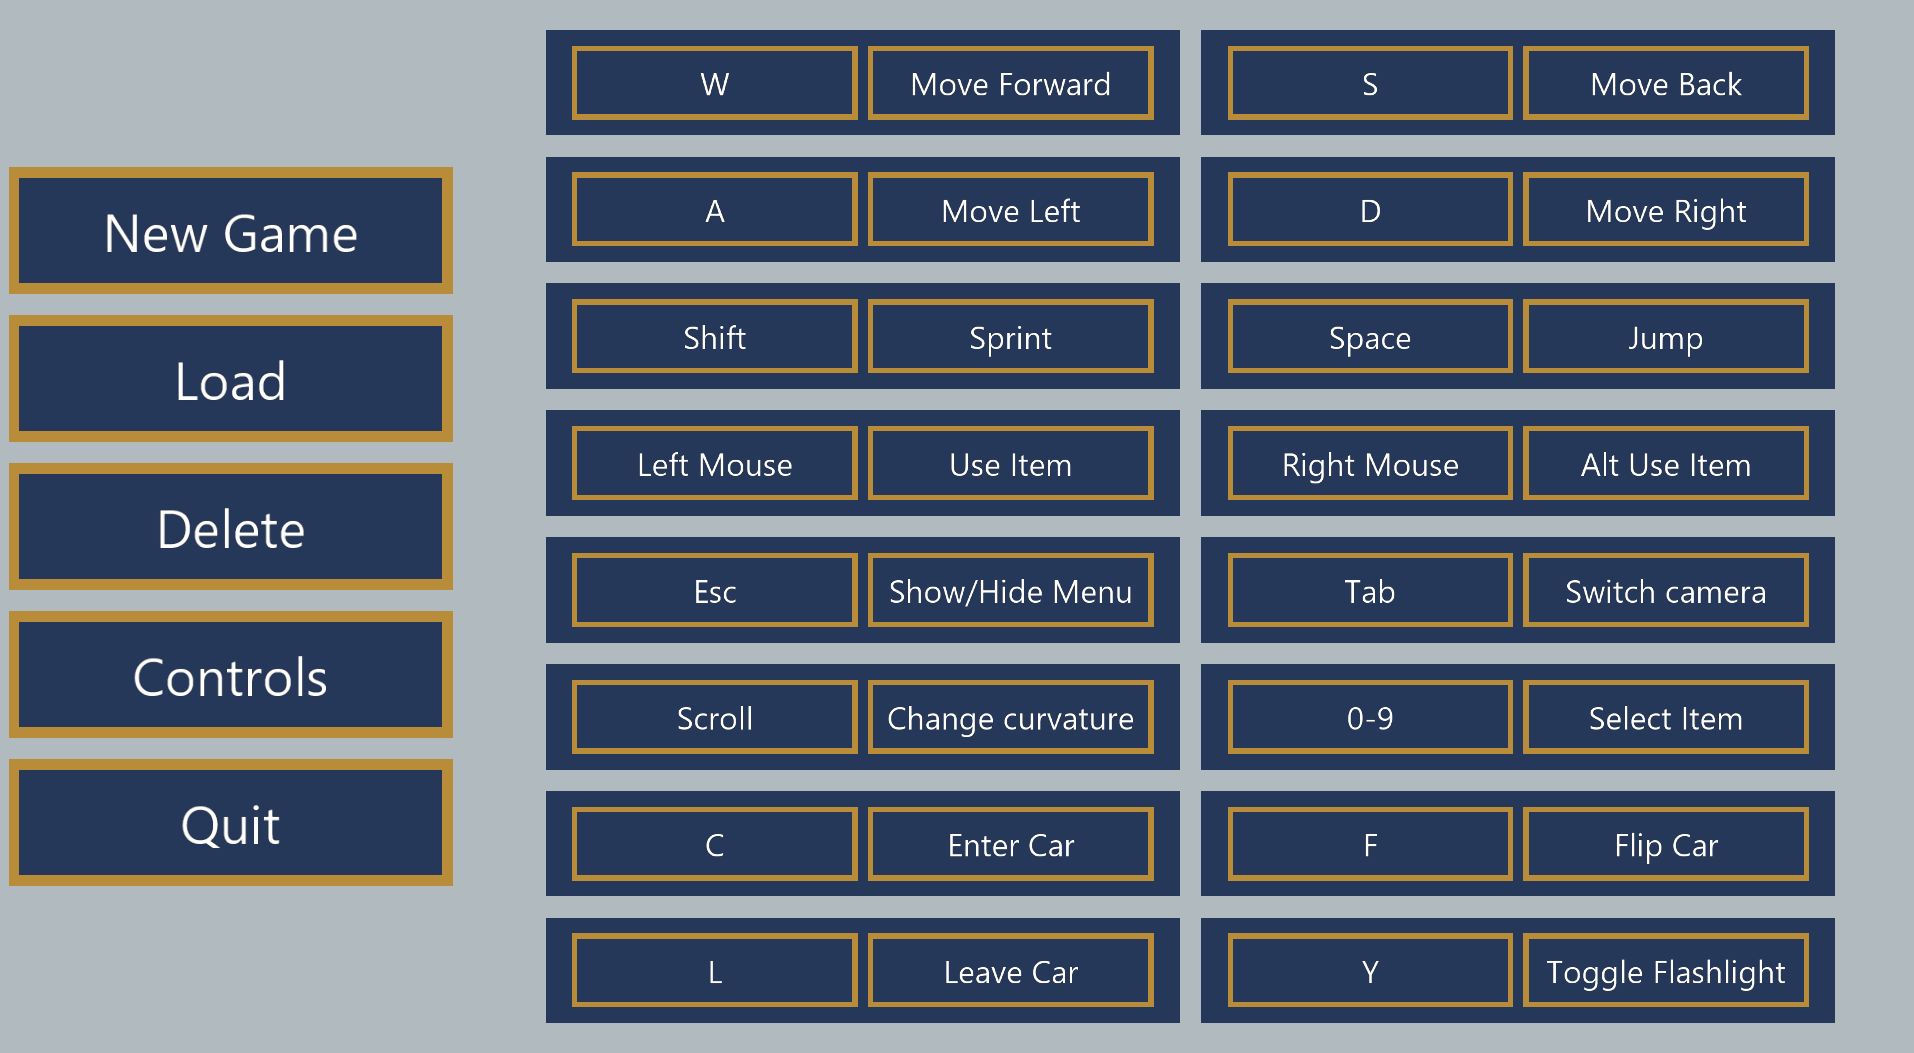
\includegraphics[width=0.8\textwidth]{chapters/user_manual/resources/controls.png}
    \caption{Controls screen}
    \label{fig:controls}
\end{figure}